\documentclass[12pt]{article}

\usepackage[utf8]{inputenc}
\usepackage[margin=1in]{geometry}
\renewcommand{\baselinestretch}{1}
\usepackage{indentfirst}

\usepackage{amsmath, amssymb}

\usepackage{graphicx}
\usepackage{float}
\graphicspath{{./figs/}}

\begin{document}

\begin{center}\begin{LARGE}
\textbf{Assignment 3: Results/Description}
\end{LARGE}\end{center}

\section*{Problem 1}

For this problem I have written three programs (\texttt{myEuler},
\texttt{myEulerPC}, and \texttt{myODEINT}) to solve the following problems.
These may be compiled all together with a \texttt{make all} as shown below.

% \begin{figure}[H]
%     \centering
%     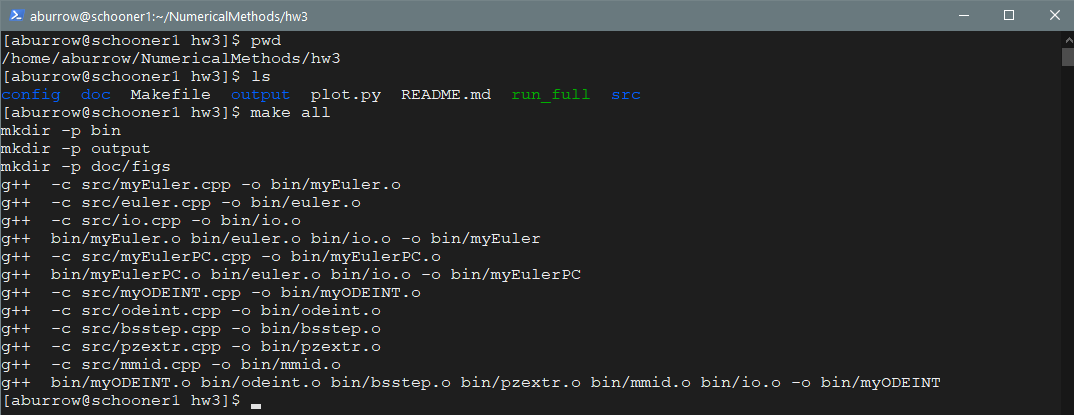
\includegraphics[width=1.0\textwidth]{compile}
%     \label{fig:compile}
% \end{figure}

\subsection*{(a)}

\begin{figure}[H]
    \centering
    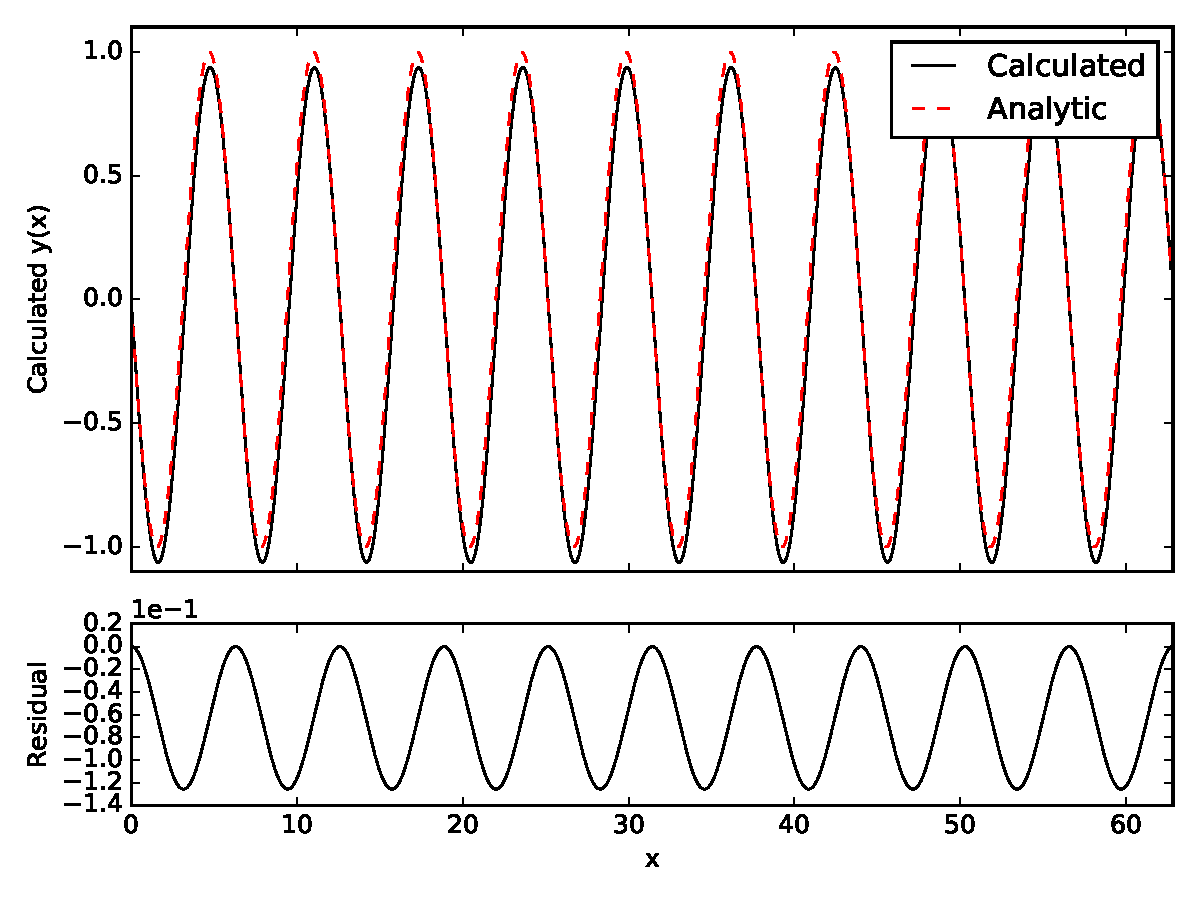
\includegraphics[scale=1]{euler}
    \label{fig:euler}
\end{figure}

\subsection*{(b)}

\begin{figure}[H]
    \centering
    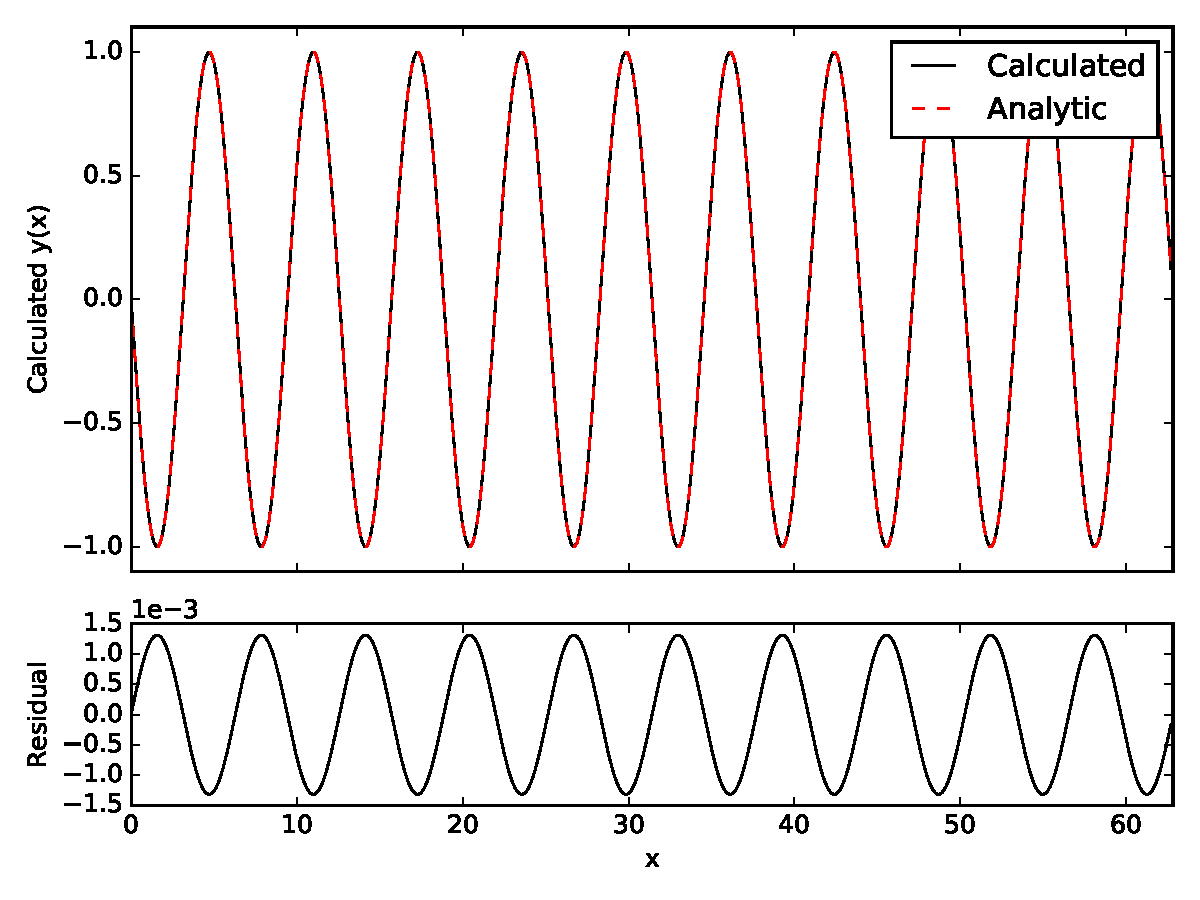
\includegraphics[scale=1]{eulerPC}
    \label{fig:eulerPC}
\end{figure}

\subsection*{(c)}

\begin{figure}[H]
    \centering
    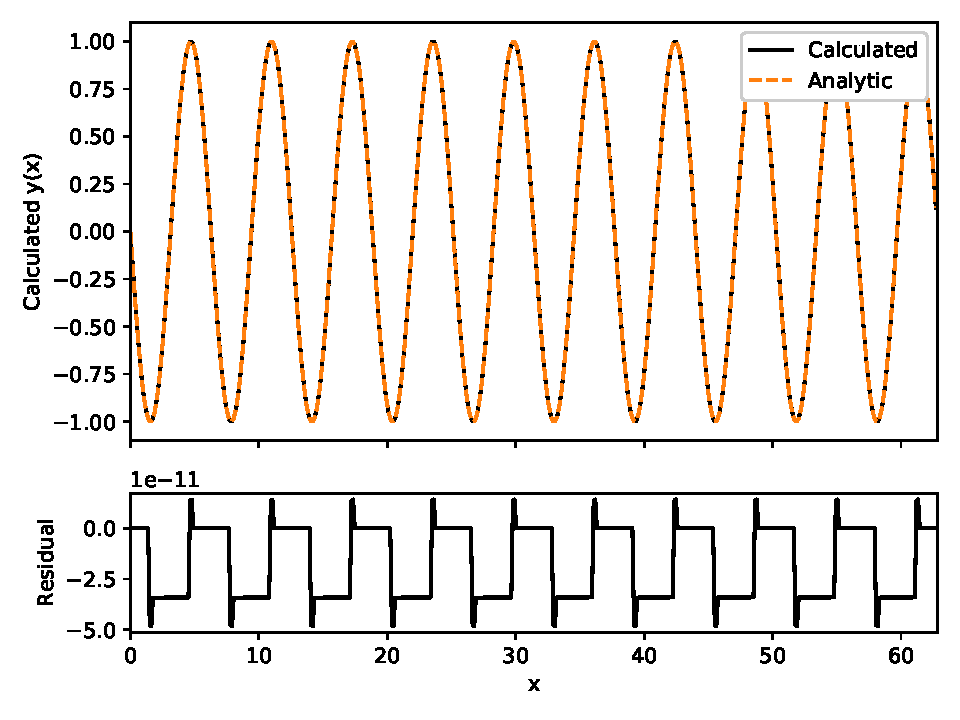
\includegraphics[scale=1]{odeint}
    \label{fig:odeint}
\end{figure}

\subsection*{(d)}



\end{document}
